\section{CPU架构选择}
  经过讨论,我们决定使用流水线架构的CPU,以获取更高的执行效率。
\section{原型通路设计}
  首先实现流水线的原型,即不对任何冲突进行优化,全部填塞气泡进行处理的CPU。
  其设计通路如图\ref{naive}所示。
  \begin{figure}[htbp]
   \centerline{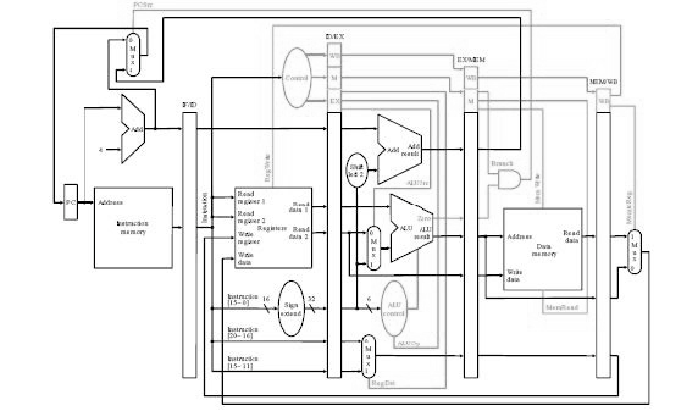
\includegraphics[width=\textwidth]{./figure/naive}}
   \caption{原型数据通路设计\label{naive}}
  \end{figure}
\section{目标通路设计}
  在有可以运行的CPU之后,需要依次添加控制、数据与跳转冲突的优化,减少气泡的出现,并添加异常处理。
  这也是本次实验的预期目标。其设计通路如图\ref{except}所示。
  \begin{figure}[htbp]
   \centerline{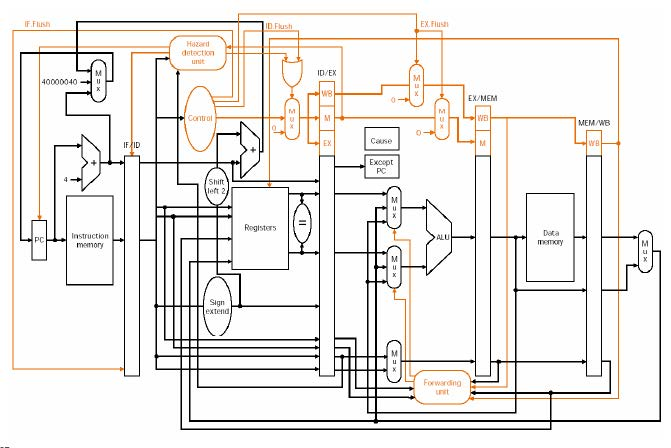
\includegraphics[width=\textwidth]{./figure/except}}
   \caption{目标数据通路设计\label{except}}
  \end{figure}
\section{拓展}
  在实现预期之后,如还有余力与兴趣,可能会添加缓存、多级缓存、集成显存等,以期获取更高的执行效率。
  但是其已经脱离CPU的设计范畴,不在此继续讨论。
